\documentclass[9pt,landscape,a4paper]{extarticle}
\usepackage[utf8]{inputenc}
\usepackage[ngerman]{babel}
\usepackage{tikz}
\usetikzlibrary{shapes,positioning,arrows,fit,calc,graphs,graphs.standard}
\usepackage[nosf]{kpfonts}
\usepackage[t1]{sourcesanspro}
%\usepackage[lf]{MyriadPro}
%\usepackage[lf,minionint]{MinionPro}
\usepackage{multicol}
\usepackage{wrapfig}
\usepackage[top=0.2mm,bottom=1mm,left=1mm,right=1mm]{geometry}
\usepackage[framemethod=tikz]{mdframed}
\usepackage{microtype}
\usepackage{bbold}
\usepackage{wrapfig}
\usepackage{amsmath} % to get \tfrac
\usepackage{xfrac} % to get \sfrac
\usepackage{dsfont} % For mathbb{1}

% START CHEATSHEET TEMPLATE

\usepackage[default]{raleway}
\usepackage{fontawesome}
\usepackage[T1]{fontenc}

\usepackage{hyperref}
\usepackage{enumitem}
\setlist[enumerate]{itemsep=0mm}
\usepackage{lipsum}

\usepackage{xcolor}
\definecolor{customcolor}{HTML}{b5e9ff}
\definecolor{alert}{HTML}{CD5C5C}
\definecolor{w3schools}{HTML}{4CAF50}
\definecolor{subbox}{gray}{0.60}
\definecolor{codecolor}{HTML}{000000}
\colorlet{xx}{customcolor}

\usepackage{paralist}

% custom commands for typsetting
\newcommand{\Prob}[0]{\mathbb{P}}
\newcommand{\Quob}[0]{\mathbb{Q}}
\newcommand{\Ex}[0]{\mathbb{E}}
\newcommand{\Var}[0]{\textup{Var}}
\newcommand{\argmin}[0]{\textup{argmin}}
\newcommand{\se}[0]{\textup{se}}

%--------------------------Editor mode.

\usepackage
[citestyle=authoryear,
sorting=nty,	  		%Sorts bibliography by year, name, title
autocite=footnote, 		%Autocite command generates footnotes
autolang=hyphen, 		
mincrossrefs=1, 	
backend=biber]
{biblatex}

\DeclareFieldFormat{postnote}{#1}
\DeclareFieldFormat{multipostnote}{#1}
\DeclareAutoCiteCommand{footnote}[f]{\footcite}{\footcites}

\bibliography{literature}
% ----------------------------------------
% --------------------------------------------------------------------------------
\usepackage{tcolorbox}

\tcbuselibrary{most,listingsutf8,minted}

\tcbset{tcbox width=auto,left=1mm,top=1mm,bottom=1mm,
right=1mm,boxsep=1mm,middle=1pt}

\newenvironment{mycolorbox}[2]{%
\begin{tcolorbox}[grow to left by=-1em,grow to right by=-1em,capture=minipage,fonttitle=\large\bfseries, enhanced jigsaw,boxsep=1mm,colback=#1!30!white,on line,tcbox width=auto, toptitle=0mm,colframe=#1,opacityback=0.7,nobeforeafter,title=#2]%
}{\end{tcolorbox}\\[0.2em]}

\newenvironment{subbox}[2]{%
\begin{tcolorbox}[capture=minipage,fonttitle=\normalsize\bfseries, enhanced jigsaw,boxsep=1mm,colback=#1!30!white,on line,tcbox width=auto,left=0.3em,top=1mm, toptitle=0mm,colframe=#1,opacityback=0.7,nobeforeafter,title=#2]\footnotesize %
}{\normalsize\end{tcolorbox}\vspace{0.1em}}

\newenvironment{multibox}[1]{%
\begin{tcbraster}[raster columns=#1,raster equal height,nobeforeafter,raster column skip=1em,raster left skip=1em,raster right skip=1em]}{\end{tcbraster}}

\newenvironment{textbox}[1]{\begin{mycolorbox}{customcolor}{#1}}{\end{mycolorbox}}

%-------------------------------
\newtcblisting{codebox}[2]{colback=white,colframe=codecolor!80!black,listing only, 
minted options={numbers=left,style=tcblatex,fontsize=\scriptsize,breaklines,autogobble,linenos=false,numbersep=1mm},
left=3mm,enhanced,breakable,boxsep=0pt,left=0pt,right=0pt,top=0pt,bottom=0pt,
title=#2, fonttitle=\bfseries,
listing engine=minted,minted language=#1}

%--------------------------------------------------------------------------------
\newcommand{\punkti}{~\lbrack\dots\rbrack~}

\renewenvironment{quote}
               {\list{\faQuoteLeft\phantom{ }}{\rightmargin\leftmargin}%
                \item\relax\scriptsize\ignorespaces}
               {\unskip\unskip\phantom{xx}\faQuoteRight\endlist}
               

%--------------------------------------------------------------------------------
\newcommand{\bgupper}[3]{\colorbox{#1}{\color{#2}\huge\bfseries\MakeUppercase{#3}}}
\newcommand{\bg}[3]{\colorbox{#1}{\bfseries\color{#2}#3}}

\newcommand{\mycommand}[2]{{\ttfamily\detokenize{#1}}~\dotfill{}~{\footnotesize #2}\\}
\newcommand{\sep}{{\scriptsize~\faCircle{ }~}}


\newcommand{\bggreen}[1]{\medskip\bgupper{w3schools}{black}{#1}\\[0.5em]}
\newcommand{\green}[1]{\smallskip\bg{w3schools}{white}{#1}\\}
\newcommand{\red}[1]{\smallskip\bg{alert}{white}{#1}\\}

\usepackage{multicol}
\setlength{\columnsep}{4pt}

\setlength{\parindent}{0pt}
\pagestyle{empty}

\usepackage{csquotes}

\newcommand{\loremipsum}{Lorem ipsum dolor sit amet.}

% END CHEATSHEET TEMPLATE

\let\bar\overline

\definecolor{myblue}{cmyk}{1,.72,0,.38}

\def\firstcircle{(0,0) circle (1.5cm)}
\def\secondcircle{(0:2cm) circle (1.5cm)}

\colorlet{circle edge}{myblue}
\colorlet{circle area}{myblue!5}

\tikzset{filled/.style={fill=circle area, draw=circle edge, thick},
    outline/.style={draw=circle edge, thick}}

\pgfdeclarelayer{background}
\pgfsetlayers{background,main}

\everymath\expandafter{\the\everymath \color{myblue}}
\everydisplay\expandafter{\the\everydisplay \color{myblue}}

\renewcommand{\baselinestretch}{.8}
\pagestyle{empty}




\makeatletter
\renewcommand{\section}{\@startsection{section}{1}{0mm}%
                                {.2ex}%
                                {.2ex}%x
                                {\color{myblue}\sffamily\small\bfseries}}
\renewcommand{\subsection}{\@startsection{subsection}{1}{0mm}%
                                {.2ex}%
                                {.2ex}%x
                                {\sffamily\bfseries}}
\makeatother

\def\multi@column@out{%
   \ifnum\outputpenalty <-\@M
   \speci@ls \else
   \ifvoid\colbreak@box\else
     \mult@info\@ne{Re-adding forced
               break(s) for splitting}%
     \setbox\@cclv\vbox{%
        \unvbox\colbreak@box
        \penalty-\@Mv\unvbox\@cclv}%
   \fi
   \splittopskip\topskip
   \splitmaxdepth\maxdepth
   \dimen@\@colroom
   \divide\skip\footins\col@number
   \ifvoid\footins \else
      \leave@mult@footins
   \fi
   \let\ifshr@kingsaved\ifshr@king
   \ifvbox \@kludgeins
     \advance \dimen@ -\ht\@kludgeins
     \ifdim \wd\@kludgeins>\z@
        \shr@nkingtrue
     \fi
   \fi
   \process@cols\mult@gfirstbox{%
%%%%% START CHANGE
\ifnum\count@=\numexpr\mult@rightbox+2\relax
          \setbox\count@\vsplit\@cclv to \dimexpr \dimen@-1cm\relax
\setbox\count@\vbox to \dimen@{\vbox to 1cm{\header}\unvbox\count@\vss}%
\else
      \setbox\count@\vsplit\@cclv to \dimen@
\fi
%%%%% END CHANGE
            \set@keptmarks
            \setbox\count@
                 \vbox to\dimen@
                  {\unvbox\count@
                   \remove@discardable@items
                   \ifshr@nking\vfill\fi}%
           }%
   \setbox\mult@rightbox
       \vsplit\@cclv to\dimen@
   \set@keptmarks
   \setbox\mult@rightbox\vbox to\dimen@
          {\unvbox\mult@rightbox
           \remove@discardable@items
           \ifshr@nking\vfill\fi}%
   \let\ifshr@king\ifshr@kingsaved
   \ifvoid\@cclv \else
       \unvbox\@cclv
       \ifnum\outputpenalty=\@M
       \else
          \penalty\outputpenalty
       \fi
       \ifvoid\footins\else
         \PackageWarning{multicol}%
          {I moved some lines to
           the next page.\MessageBreak
           Footnotes on page
           \thepage\space might be wrong}%
       \fi
       \ifnum \c@tracingmulticols>\thr@@
                    \hrule\allowbreak \fi
   \fi
   \ifx\@empty\kept@firstmark
      \let\firstmark\kept@topmark
      \let\botmark\kept@topmark
   \else
      \let\firstmark\kept@firstmark
      \let\botmark\kept@botmark
   \fi
   \let\topmark\kept@topmark
   \mult@info\tw@
        {Use kept top mark:\MessageBreak
          \meaning\kept@topmark
         \MessageBreak
         Use kept first mark:\MessageBreak
          \meaning\kept@firstmark
        \MessageBreak
         Use kept bot mark:\MessageBreak
          \meaning\kept@botmark
        \MessageBreak
         Produce first mark:\MessageBreak
          \meaning\firstmark
        \MessageBreak
        Produce bot mark:\MessageBreak
          \meaning\botmark
         \@gobbletwo}%
   \setbox\@cclv\vbox{\unvbox\partial@page
                      \page@sofar}%
   \@makecol\@outputpage
     \global\let\kept@topmark\botmark
     \global\let\kept@firstmark\@empty
     \global\let\kept@botmark\@empty
     \mult@info\tw@
        {(Re)Init top mark:\MessageBreak
         \meaning\kept@topmark
         \@gobbletwo}%
   \global\@colroom\@colht
   \global \@mparbottom \z@
   \process@deferreds
   \@whilesw\if@fcolmade\fi{\@outputpage
      \global\@colroom\@colht
      \process@deferreds}%
   \mult@info\@ne
     {Colroom:\MessageBreak
      \the\@colht\space
              after float space removed
              = \the\@colroom \@gobble}%
    \set@mult@vsize \global
  \fi}

\makeatother
\setlength{\parindent}{0pt}

\begin{document}
\begin{multicols*}{4}
\scriptsize
\section*{Linear Regression}
$y_i = \beta_1 x_{i1}+...+\beta_p x_{ip} + \epsilon_i$ (note: $x_{i1}\equiv 1$, so $\beta_1$ is intercept) where $\epsilon_1,...,\epsilon_n$ independent, $E(\epsilon_1)=0, \text{Var} (\epsilon_i)=\sigma^2$ (homoscedasticity)

\textbf{LSE:} $\hat \beta = \text{argmin}_\beta ||Y-Xb||_2^2 = (X^\top X)^{-1}X^\top Y \sim \mathcal{N}_p(\beta, \sigma^2 (X^\top X)^{-1})$ \\
$\hat \sigma^2 \approx \frac 1 {n-p}RSS$
also if error Gaussian then: $\hat Y \sim \mathcal{N}_n(X\beta, \sigma^2 P)$, error\\
$e \sim \mathcal{N}_n(0, \sigma^2(I-P))$,
$\hat \sigma^2 \sim {\sigma^2 }/{(n-p)}\cdot X_{n-p}$
where $P=X(X^\top X)^{-1}X^\top $

\textbf{Categorical Variables:} 
For two levels:$y_i = \beta_1 x_{i1}+...+\beta_p x_{ip} + \lambda d_{is} + \epsilon_i$ 
so if $i$ is in category, then $d_{is}=1$ else $d_{is}=0$. This acts as a different intercept ($E(y_i)-E(y_j)=\lambda$). If more categories, add more dummy variables.

\textbf{Interaction:} dummy can also influence slope: add term $\delta d_i x_i$, can influence interaction between predictors: add term $\delta x_{i2} x_{i3}$, can influence other categorical variable: add term $\delta d_{i1}d_{i2}$.

\subsection*{Measuring Goodness of Fit}
$H_0: y = X\beta + \epsilon$ with $\beta_j=0$
$H_A: y = X\beta + \epsilon$ with $\beta_j\neq 0$\\
Under $H_0: \frac{\hat \beta_j - (E[\hat \beta_j]=0)}{\sqrt{\sigma^2(X^\top X)^{-1}_{jj}}} \sim \mathcal{N}(0,1)$
t-statistic: $\frac{\hat \beta_j}{\sqrt{\hat \sigma^2 (X^\top X)^{-1}_{jj}}} \sim t_{n-p}$
\textbf{P-Value:} P(obs. a value of the test stat. that is as extreme or more extreme than the one we saw if $H_0$ is true).
If $< \alpha$ then reject $H_0$.
% Too lazy to draw this in LaTeX ;)
\includegraphics[width=0.7\linewidth]{interaction.PNG}

\begin{codebox}{r}{Linear Regression}
fit <- lm(y~x1+x2) # Fit only x1 and x2 (so p=3)
predict(fit, pred.data.frame)
# Manual fit
X <- cbind(1, x1, x2) # p = 3
XtX.inv <- solve(t(X) %*% X)
beta.hat <- XtX.inv %*% t(X.int) %*% y
res <- y - X.int %*% beta.hat # Residuals
RSE <- sqrt(sum(res^2)/(n-p)) # Residual std. error. Est. of the sd of the noise in the linear model
se.x1 <- RSE * sqrt(XtX.inv[2, 2]) # Std. error of x1
t.val.x1 <- beta.hat[2] / se.x1 # T value of x1
p.val.x1 <- 2*pt(abs(t.val.x1), df=n-p, lower=F)
# R squared: proportion of Var(y) that is explained by the fitted linear model.
RSE <- sqrt(sum(residuals(fit)^2)/(n-p))
RSS <- sum(res^2) # Residual sum of squares
TSS <- sum((y - mean(y))^2) # Total sum of squares
R.sq <- 1 - RSS / TSS
AdjR2 <- 1 - (RSS/(n-p))/(TSS/(n-1))
# Alternative t-value
coef <- summary(fit1)$coefficients
t1 <- coef["x1","Estimate"]/coef["x1","Std. Error"]
# Finding p-values
fit.smaller <- lm(y ~ x1)
anova(fit.smaller, fit, fit.all)
# Overall F-Test
fit.empty <- lm(y ~ 1, data=...) # Empty model
anova(fit.empty, fit) # Compare models
# Alternative F-test
Ftest <- summary(fit)$fstatistic
pval <- 1 - pf(Ftest[1], df1=Ftest[2], df2=Ftest[3])
# Categ. var. by hand & LOOCV
a1 <- (levels(shelveloc)[2]==shelveloc)*1
lcv<-mean((residuals(fit)/(1-lm.influence(fit)$h))^2)
\end{codebox}

\textbf{R Diagnostic plots: } \#1 Tukey-Anscombe Plot the points follow the line, else $E(\epsilon)=0$ violated. \#2 Q-Q Plot should follow line, else error not Gaussian (still all fine). \#3 Scale-Location: should be flat, else $\text{Var}(\epsilon_i)=\sigma^2$ violated (p-values wrong). \#4/\#5 Cook distance: shows if some data points have a larger impact on the fit than others (outliers). Note: cannot detect if the residuals are correlated with these plots!
\section*{Tests \& Confidence Intervals}
Want to calculate: $P\left( t_{\alpha / 2, n-p} < \sfrac{\hat \beta_j - \beta_j} {\hat {se}(\hat \beta_j)} < t_{1-\alpha / 2, n-p} \right) = 1 - \alpha$.
$CI = \hat \beta_j \pm \hat se(\hat \beta_j) \cdot t_{1- \alpha / 2, n-p} = \hat \beta_j \pm \hat \sigma \sqrt{x_0^\top (X^\top X)^{-1} x_0} \cdot t_{1- \alpha / 2, n-p}$
\subsection*{Prediction Interval}
For new point $x_0$:
$\hat y_0 = x_0^\top \beta \pm \hat \sigma^2 \sqrt{1 + x_0^\top (X^\top X)^{-1}x_0} \cdot t_{1-\alpha / 2, n-p}$

\textbf{P-Value:} P(obs. a value of the test stat. that is as extreme or more extreme than the one we saw if $H_0$ is true).
If $p < \alpha$, reject $H_0$.

% Too lazy to draw this in LaTeX ;)
\includegraphics[width=0.7\linewidth]{img/interaction.PNG}

\subsection*{Bias Variance Trade-Off}
Expected Test MSE at $x_0$: $\Ex[(y_0 - \hat f(x_0)^2] = \text{Bias}^2 (\hat f(x_0)) + \text{Var}(\hat f(x_0)) + \sigma^2$, where $\text{Bias}^2(\hat f(x_0)) = (f(x_0)-\Ex[\hat f(x_0)])^2$, $Bias = \Ex[\hat f(x_0)] - f(x_0)$ (see code).

\textbf{Notation}
$Y_i=f(X_i)+\epsilon_i$, where $\epsilon_i$ iid, $\Ex[\epsilon_i]=0$, $\Var(\epsilon_i)=\sigma^2$. $f$ is arbitrary fixed unknown function. Consider estimator $\hat f$ trained/fitted on $(x_1,y_1),...,(x_n,y_n)$. Then Training MSE: $\tfrac{1}{n} \sum_{i=1}^n (y_i-\hat f(x_i))^2$. Test MSE on new sample $(\tilde x_1, \tilde y_1),...,(\tilde x_m, \tilde y_m)$: $\tfrac{1}{m}\sum_{i=1}^m (\tilde y_i-\hat f(\tilde x_i))^2$.

\textbf{Trade off}
Consider new pair $(x_0,y_0)$: Then $\Ex[(y_0-\hat f(x_0))^2]=(f(x_0)-\Ex[\hat f(x_0)])^2+\Var(\hat f(x_0))+\Var(\epsilon)=(\textup{Bias}(\hat f(x_0)))^2+\Var(\hat f(x_0))+{\sigma^2}$, $\sigma^2$ irreducable error, where Exp. is over different training sets.

\begin{codebox}{r}{Confidence Intervals \& p-value}
  # P-value: variant 1, 1 sided, H0: <= 6
  res <-  replicate(nsimul, simulateSomething())
  pval.1 <- (1+sum(res.1 <= 6))/(nsimul+1)
  # P-value, V2. (V3: t.test(...), V4: pnorm(...))
  pval.2 <- 2*pt(qt(1-alpha/2,n-p), df=n-p, lower=FALSE)
  confint(fit) # Automatic CI.
  # Manual CI (for intercept):
  se.intercept <- summary(fit)$coef[1,2]
    coef(fit)[1] - qt(.975, n-2)*se.intercept
    coef(fit)[1] + qt(.975, n-2)*se.intercept
    # Predict value and C.I. (c for $\Ex[Y_0]$, p for $Y_0$):
    # Automatic Prediction CI
    predict(fit,newdata=data.frame(name=5), level=.95, interval="p")
    # Automatic CI
    predict(fit,newdata=data.frame(name=5), level=.95, interval="c")
    # Manual Prediction CI
    fitted <- fit$coef[1] + fit$coef[2]*x0
    quant <- qt(.975,n-2) # Quantile of t distribution
    sigma.hat <- sqrt(sum((fit$resid)^2/(n-2)))
  X <- as.matrix(cbind(1,thuesen[,1]))
  XtXi <- solve(t(X) %*% X) # (X^T X)^{-1}
  X00 <- as.matrix(c(1,x0), nrow=2)
  se <- sigma.hat * sqrt(t(X00) %*% XtXi %*% x00)
  lower <- fitted - quant * se
  upper <- fitted + quant * se
  # Bias Variance Trade-Off of a Method
  Bias <- mean(EstimateUsingCV) - TrueValueSimulated
  MSE <- Bias^2 + var(EstimateUsingCV)
\end{codebox}

\section*{K Nearest Neighbors}
Non-parametric method: $\hat f(x)=1/k \sum_i yi$ where $y_i$ are the $k$ nearest neighbors of $x$. If $k$ is larger has less variance, more bias. If $k$ is smaller has more variance, less bias.
Fails if there are lots of useless predictors.

\begin{codebox}{r}{KNN}
library(kknn)
dfTrain=data.frame(y=Ytrain,x=Xtrain)
dfTest=data.frame(x=Xtest)
fit.kknn <- kknn(y ~ ., dfTrain,dfTest,k=8)
predTest=predict(fit.kknn) # predictions on dfTest
library(class) # Alternative library for knn
knn(train, test, k=5)
\end{codebox}
\section*{Cross Validation}
Can be used for \textit{model assessment} (estimate test MSE) and \textit{model selection} (choose tuning parameters, variable selection). But not both at the same time (use double CV instead). \\
\textbf{Validation set:} split data into two halves, train on one, test on the other (most bias).
\textbf{k-Fold:} same, but with many folds. Try all folds for test and average metrics over the folds (in between). $\text{Var}(\hat {\theta_k}) = 1/K \cdot \hat {\text{Var}}(MSEs)$ \textbf{LOOCV:} extreme version where each data point is a fold (least bias). \\
$\theta_k = \frac 1 k \sum_{i=1}^k \frac 1 {|I_k|} \sum_{i\in I_k} (y_i - \hat f^{-I_k}(x_i))^2$, 
$\theta_{L} = \frac 1 n \sum_{i=1}^n (y_i - \hat f^{-i}(x_i))^2$
\section*{Bootstrap}
Sample uniform from data points with replacement, compute bootstrapped estimator. 
For a large dataset $x_1, ..., x_n$ the probability that $x_1$ is contained in a random bootstrap dataset is:
$1-(1-1/n)^n \approx 2/3$ (for large $n$, limit goes to $1-1/e$).

\subsection*{Bootstrap Consistency}
For an increasing sequence $a_n$ (often $\sqrt{n}$) where $a_n^{-1}$ is the convergence rate of $\hat \theta_n$:
$P(a_n(\hat \theta_n - \theta) \leq x) - P^*(a_n(\hat \theta_n - \hat \theta_n) \leq x) \to^P 0$ as $n\to \infty$. 
This holds when $\sqrt{n}(\hat \theta_n - \theta)$ is asympt. normal. 
Allows to estimate $\text{Bias}(\hat \theta_n) = E[\hat \theta_n] - \theta$ by $E^*[\hat \theta^*_n] - \hat \theta_n \approx \bar{\hat{\theta}^*_n} - \hat{\theta}_n$. Can also estimate $\text{Var}^*(\hat\theta_n)$ by $\text{Var}^*(\hat\theta^*_n)$ .
With bootstrap consistency, we have $\sfrac{\Var^\ast(\hat\theta_n^\ast)}{\Var(\hat\theta_n)}\stackrel{P}{\rightarrow}1$ 
and $\sfrac{\Ex^\ast[\hat\theta_n^\ast]-\hat\theta_n}{\Ex[\hat\theta_n]-\theta}\stackrel{P}{\rightarrow}1$.
%(Inconsistency can occur if parameter is on the boundary of the parameter space/$\mu=0$.)

\textbf{Resersed Quantile Bootstrap CI:} $[\hat \theta_n - Q_{\hat \theta^* - \hat \theta}(1- \alpha / 2), \hat \theta_n - Q_{\hat \theta^* - \hat \theta}(\alpha / 2)]$ (type="basic"), \textbf{Normal Bootstrap CI:} Assums $\hat\theta_n$ to be asympt. normal: $\hat\theta_n \pm Q_z(1-\alpha / 2)\hat{sd}(\hat\theta_n)$ where $z \sim \mathcal{N}(0,1)$ and $\hat{sd}(\hat\theta_n)=\sqrt ({\text{Var}(\hat\theta_n^*)})$ (type="norm"), \textbf{Quantile Bootstrap CI:} not theoret. justified unless $\hat\theta_n$ is symm.:
$[Q_{\theta_n^*}(\alpha / 2), Q_{\theta_n^*}(1-\alpha / 2)]$ (type="perc"). 
Same as \textit{reversed quantile bootstrap CI} if $\hat\theta_n^* - \hat\theta_n$ is symm. around 0, 
\textbf{Bootstrap T:} Rely on $t=\sfrac{\hat\theta_n -\theta}{\hat {sd}(\hat\theta_n)}$ and $t*=\sfrac{\hat\theta_n^*-\hat\theta_n}{\hat{sd}(\hat\theta_n^*)}$ to be asympt. equal: 
$[\hat\theta_n - \hat{sd}(\hat\theta_n) \cdot Q_{t*}(1-\alpha / 2), \hat\theta_n - \hat{sd}(\hat\theta_n) \cdot Q_{t*}(\alpha / 2)]$. 
Note: $\hat{sd}(\hat\theta_n)$ is computed as above and $\hat{sd}(\hat\theta^*_n)$ is computed using a 2nd layer bootstrap.

\textbf{Parametric Bootstrap:}
Assume data is generated by some parametric distr. (e.g. $\mathcal{N}(\mu, \sigma^2)$), est. the param.,
then create new data sets from this distr. (with or whithout replacement). Works only well if distr. is approx. correct.
Pros: good if parametric model is approximately true. Cons: Bad if not. (then non-param. bootstrap [with replacement] is better).

\textbf{Smoothed Bootstrap:}
Given data $Z_1,...,Z_n \sim_{i.i.d} P$, we estimate $P$ by some smooth (non-parametric) estimate $\tilde P_n$, then generate bootstrap samples from $\tilde P_n$. In between non-param. and param. bootstrap. Works well if $P$ is indeed smooth.

\textbf{Confidence intervals:}
Quantile: $[q_{\hat\theta_n^\ast}(\alpha/2), q_{\hat\theta_n^\ast}(1-\alpha/2)]$ Same as Rev. quant. if distr. of $\hat\theta_n^\ast-\hat\theta_n$ is symm. In R: \texttt{perc}.

Normal: $\hat\theta_n \pm q_Z(1-\alpha/2)\widehat{\textup{sd}}(\hat\theta_n)$, where $Z\sim N(0,1)$, $\textup{sd}(\hat\theta_n)=\sqrt{\widehat{\Var}^\ast(\hat\theta_n^\ast)}$. In R: \texttt{norm}

Reversed quantile: $[\hat\theta_n-q_{\hat\theta_n^\ast-\hat\theta_n}(1-\alpha /2), \hat\theta_n-q_{\hat\theta_n^\ast-\hat\theta_n}(\alpha /2)]=[2\hat\theta_n-q_{\hat\theta_n^\ast}(1-\alpha/2), 2\hat\theta_n-q_{\hat\theta_n^\ast}(\alpha/2)]$. In R: \texttt{basic}

Bootstrap T: $[\hat\theta_n-q_{\sfrac{\hat\theta_n^\ast-\hat\theta_n}{\widehat{\textup{sd}}(\hat\theta_n^\ast)}}(1-\alpha/2)\widehat{\textup{sd}}(\hat\theta_n), \hat\theta_n-q_{\sfrac{\hat\theta_n^\ast-\hat\theta_n}{\widehat{\textup{sd}}(\hat\theta_n^\ast)}}(\alpha/2)\widehat{\textup{sd}}(\hat\theta_n)]$, where $\widehat{\textup{sd}}(\hat\theta_n^\ast)$ is obtained via second layer of bootstrap. In R: \texttt{stud}.
\textbf{Bootstrap for regression:}
Model: $\Ex[Y|X=x]=\mu(x)$. Let $\hat\mu(x)$ be an estimate of $\mu(x)$. Let $r_i=y_i-\hat\mu(x_i)$ denote the residuals. Different options:

-Simulate new $X$-values from the model's estimated distribution for $X$. Then draw $Y$-values from the model's estimated distribution of $Y|X$.

-Hold the $x$'s fixed, and draw $Y|X$ from the model's estimated distribution of $Y|X$.

-Hold the $x$'s fixed and set $Y=\hat\mu(x)$ plus a randomly resampled residual $r_j$.

-Resample $(x_i,y_i)$ pairs.

Options range from fully parametric to fully non parametric.

\begin{codebox}{r}{Bootstrap}
   library(boot)
   sample(c(1:n), n, replace=T) # bootstrap sample
   res.boot <- boot(Portfolio, f, R=1000)# f's args: (data, idx)
   res.boot$t0 # Estimates on original data
   res.boot$t # Estimates on bootstrapped data
   # Confidence intervals for variable i
   boot.ci(res.boot, type="basic", index=i)
   # Example to find all confidence intervals
   tm <- function(x, ind) {mean(x[ind], trim = 0.1)}
   tmv <- function(x, ind) {
      # bootstrap Var, required for the bootstrap T CI
      t2 <- var(boot(data=x[ind], statistic=tm, R=50)$t)
      return(c(tm(x, ind), t2)) }
   res<-boot(data=..,statistic=tmv,R=10,sim="ordinary")
   boot.ci(res, conf=0.95, type=c("basic","norm", "perc","stud"), var.t0=var(res.boot$t[,1]))
   # Intervals by hand (t0: estimate, t: bootstrapped)
   quantile.CI <- quantile(t,probs=c(0.025,0.975))
   norm<-c(t0-qnorm(0.975)*sd(t),t0+qnorm(0.975)*sd(t))
   reversed.CI <- t0-quantile(t-t0,probs=c(0.975,0.025))
   # Parametric Bootstrap
   # f1 is the bootstrap function: args (data)
   # f2 returns a random dataset: args (data, mle)
   res.boot <- boot(data, f1, R=1000, ran.gen=f2, sim="parametric",  mle=1/mean(x1))
\end{codebox}

\section*{Permutation Test}
\textbf{Pros/Cons}
- Advantages: Idea is simple and elegant, flexible, no parametric/distribution assumption, use any test statistic, $p$-values and type I error control are exact, not asymptotic (if all permut. are considered).

- Limitations: Need computational power; not everything can be formulated as perm. test. (example: indiv. coefficients in regression).

\textbf{Paired/unpaired two sample} Paired: two measurements on same object/person, etc.
\textbf{Parametric vs. non parametric tests} Parametric: assumes form of distribution, e.g. T-test. Non parametric: No assumption about distribution, e.g. Wilcoxon rank sum test, Randomization/permutation tests.
Non-parametric, simple model that works with any test statistic. P-values and type I error control exact/approximate (not asymptotic), but needs computational power and not everything can be modeled in this way (e.g. individual coefficients in LR)

{1. Pick a test stat. that measures some difference between groups}

  {2. Consider all possible permutations (or randomly permute) to obtain a permutation distribution.}

  {3. Compare observed value to permutation distribution}


\subsection*{Wilcoxon Test}
Non-parametric, unpaired, robust test. $H_0: F_1 = F_2$, $H_A: F_1 $ shifted compared to $F_2$. Compute ranks of randomly switched sign (different group assignment), reject $H_0$ if observed rank over critical value of rank distribution.
Determine the ranks of all data points $(1,...,n_1+n_2)$. Compute $U$: sum of ranks in one group. Distr. of $U$ under $H_0$ in $R$ or simulate: Permute $Y$ values among two groups in all possible ways (or simulate large number). For each such group assignement compute the sum of ranks in one group. Idea: under $H_0$ treatment has no effect, thus assignment has no effect.

Wilcoxon signed rank test: $V=\sum_i \text{rank}(|D_i|)\cdot 1_{D_i > 0}$. $D_i$ difference on ith object.

\begin{codebox}{r}{Permutation Test \& Wilcoxon Signed Rank Sum Test}
  # Permutation test
  fit <- lm(y~X)
  obsF <- summary(fit)$fstatistic[1]
    res.f <- rep(NA, 10000)
    for (i in 1:10000){
        y <- y[sample(1:nrow(X), nrow(X))]
        fit.tmp <- lm(y~X)
        res.f[i] <- summary(fit.tmp)$fstatistic[1]
      }
    pval<-(sum(obsF<=res.f,na.rm=T)+1)/(length(res.f)+1)
    # Permutation Wilcoxon Signed Rank Sum Test
    diff <- immer$Y1 - immer$Y2
  V.obs <- sum(rank(abs(diff)) * (diff > 0))
  V <- numeric(100000)
  for(i in 1:100000){
      perm<-diff * sample(c(1,-1),nrow(immer),replace=T)
      V[i] <- sum(rank(abs(perm)) * (perm > 0))
    }
  p.value <- table(V >= V.obs)["TRUE"]/length(V)
  # Automatic
  wilcox.test(diff, alternative = "greater")
  wilcox.test(control, treatment , alternative = c("two.sided", "less", "greater") # for unpaired two sample Wilc. test.
\end{codebox}

% Maybe drop this
%\subsection*{Exercise Wilcoxon}
%Let $X_1,...,X_m~F_X$ and $Y_1,...,Y_m~F_Y$ be independent. $H_0: F_X=F_Y$, $H_A: F_X(x) = F_Y(x-a) \  \forall x$ and $a>0$. Let $D_i = X_i - Y_i, i \in [1,m]$. Show that $H_0$ and $H_A$ can be written as $H_0: $ the distribution of $D$ is symmetric around $a=0$, $H_A$ the distribution of $D$ is symmetric around $a>0$. 

%We show that the distribution of $D$ is symmetric around $a$: $P(D-a \leq d) = P(-(D-a) \leq d)$. We have $P(D-a \leq d) = P(D \leq d + a) = \int P(X-Y \leq d+a |Y=y) f_Y(y) dy = \int P(X-y \leq d+a) f_Y(y) dy = \int P(X \leq d+a+y) f_Y(y) dy = \int F_X(d+a+y)f_Y(y)dy$ We get the same when exchanging $X$ and $Y$: $P(-(D-a)\leq d) = P(-D \leq d-a) = P(Y-X \leq d-a) = \int F_Y(d-a+x)f_X(x)dx$. 

%We can use that $F_X(x)=F_Y(x-a)$ and $f_X(x)=f_Y(x-a)$ to show: $\int F_X(d+a+y)f_Y(y)dy = \int F_Y(d+a+y-a)f_X(y+a)dy = \int F_Y(d+y)f_X(y+a)dy = \int F_Y(d-a-x)f_X(x)dx$

\section*{Multiple Testing}

\begin{tabular}{l|l|l|l}
 & \textbf{$\mathbf{H_0}$ true} & \textbf{$\mathbf{H_A}$ true} &  \\ \hline
$\mathbf{H_0}$ \textbf{not reject.} & $U$ \textcolor{green}{true neg.} & \begin{tabular}[c]{@{}l@{}}$T$ \textcolor{red}{false neg.} \\ Type II error\end{tabular} & $m-R$ \\ \hline
$\mathbf{H_0}$ \textbf{reject.} & \begin{tabular}[c]{@{}l@{}}$V$ \textcolor{red}{false pos.} \\  Type I error\end{tabular} & $S$ \textcolor{green}{true pos.} & $R=V+S$ \\ \hline
 & $m_0$ & $m-m_0$ & $m$
\end{tabular}

Capital letters represent RV. Only $R$ is observable. $m$ is fixed and known, $m_0$ is fixed and unknown. 
If $m_0=m$ then \textit{global null}. 

$P(\textit{type I error}) = P(\textit{rejecting } H_0 \textit{ when } H_0 \textit{ is true}) = \alpha$ 

$P(\textit{type II error}) = P(\textit{not rejecting } H_0 \textit{ when } H_A \textit{ is true}) = \beta$ 

\textbf{Power of a test} $1-\beta$ 
\textbf{False discovery proportion (FDP):} $Q=V/R$ (note: $V/R=0$ if $V=R=0$) 
\textbf{False discovery rate (FDR):} $E(Q)$ Expected proportion of false discoveries among all disc. 
\textbf{Family wise error rate (FWER):} $P(V\geq 1)$ Prob. of making one or more false discoveries. 
Note: controlling the FWER is more strict than controlling the FDR: 
if $V\geq 1$, then $Q=V/R \leq 1$ and if $V=0$, then $Q=V/R=0$. So $\mathds{1}_{\{V\geq 1\}}\geq Q$: $\text{FWER}=P(V\geq 1)=E[\mathds{1}_{\{V\geq 1\}} \geq E[Q] = \text{FDR}$. 
If $m=m_0$/under global null, then $\text{FWER}=\text{FDR}$. Generaly, $\alpha m \geq \text{FWER}\geq\text{FDR}$.

\subsection*{Bonferroni Correction}
Idea: $\text{FWER}=P(V\geq 1)=P(\textit{at least one false rejection among tests }\allowbreak T_1,...,T_m)=P(\cup_{i=1}^m\{\textit{false rejection in test }T_i\}) \leq \sum_{i=1}^m P(\{\textit{false rej.} \allowbreak \textit{ in test}\}) \leq \sum_{i=1}^m \alpha = m\cdot \alpha$ 
so we set the signif. level of individual tests to $\alpha' =\alpha /m$ (or, equiv.: $p_{bonf} = min(1, n\cdot p)$), then $\text{FWER}\leq m\alpha' =\alpha$. 
\textbf{Power:} if the tests are indep. and $m=m_0$ then $\text{FWER}=1-(1-\alpha)^m$ which is $\approx \alpha\cdot m$ for small $\alpha$ and moderate $m$. 
If the tests are dependent/correlated: too conservative.

\subsection*{Benjamini-Hochberg}
Let $p(1)\leq p(2) \leq ... \leq p(m)$ be ordered p-values. Let $i_0$ be the largest $i$, s.t. $p(i)\leq q\cdot i / m$. 
Reject all $H_{(i)}$ with $i\leq i_0$. For independent test statistics (or p-values) this controls the $\text{FDR}$ at level $q$, i.e. $\text{FDR}=q\cdot m_0 / m \leq q$. 

\subsection*{Westfall Young Permutation Procedure}
Provides \textit{weak control of the FWER} (i.e. under the global null). 

Given a data $X \in \mathbb{R}^{n\times (m+1)}$ size and $y\in \{0,1\}^n$. 
If $m=m_0$ then one can permute the y-values:

1. Repeat many times: premute y-cols, do a two sample test (e.g. Wilcoxon) for each $x_j$ col. (comparing $x_j[y==1]$ and $x_j[y==0]$). Let $p_j$ for $j=0,...,m$ be the corresp. p-value. Store $\min(p_1,...,p_m)$.

2. Set $\delta$ to the empirical $\alpha$-quantile of the permutation distribution of $min(p_1,...,p_m)$. 

3. Reject any null hypothesis where the two-sample test on the original data has p-value $\leq \delta$.


\begin{codebox}{r}{Westfall Young Permutation Procedure}
nr.sim <- 1000
min.p.values <- numeric(nr.sim)
for(sim in 1:nr.sim) {
  y_perm = sample(y, length(y), replace = FALSE)
  min.p.values[sim] <- min(apply(x, 2, function(j) chisq.test(x = j, y = y_perm)$p.value))
}
delta <- quantile(min.p.values, probs = 0.05)
table(p.values < delta)
\end{codebox}

\section*{Model Selection}
Criteria for model selection (for linear models): 
$\text{Mallow's }C_p=\tfrac 1 n (RSS + 2d\cdot \hat\sigma^2)$, 
$AIC = \tfrac{1}{n\hat\sigma^2}(RSS+2d\cdot\hat\sigma^2)$, 
$BIC= \tfrac{1}{n\hat\sigma^2}(RSS+\log(n)d\cdot\hat\sigma^2) = -2 \cdot\log(\hat L) + d\cdot\log(n)$, 
where $\hat L$ is the maximized value of the likelihood of the model, 
$n$: sample size, $d$: nr. of params in model, $AdjR^2=1-\tfrac{RSS / (n-d-1)}{TSS / (n-1)}$.

\subsection*{Shrinkage Methods}
Less variance, more bias.
Assume centered variable (no intercept).
Remark: Ridge does not really do model selection, Lasso does, since $L^1$-spheres have "corners" (i.e. variables can $\rightarrow 0$). 
Ridge though has an analytic solution. 
Note: standardize variables to have scale invariance/variance $= 1$: $\tilde x_{ij}=\sfrac{x_{ij}}{\sqrt{\tfrac{1}{n} \sum_i(x_{ij}- \bar x_j)^2}}$
\textbf{Ridge regression:} $\hat\beta_s^{ridge} = \text{argmin}_\beta RSS(\beta) + \lambda ||\beta||_2^2 = (X^\top X + \lambda I)^{-1}X^\top y$ (if $X$- matrix has no intercept (i.e. center variables before))
\textbf{Lasso:} 
$\hat\beta_s^{lasso}\text{argmin}_\beta RSS(\beta) + \lambda ||\beta||_1$,
\textbf{Elastic Net:} $\hat\beta_s^{elastic} = \text{argmin}_\beta RSS(\beta)+(1-\alpha)\lambda||\beta||_1 + \alpha \lambda ||\beta||_2^2$($\alpha=1$: ridge, $\alpha=0$: lasso),

\textbf{Adaptive Lasso:} Lasso with penalty weights:

$\hat\beta_s^{adapt.lasso}\text{argmin}_\beta RSS(\beta) + \lambda \sum_{j=1}^p w_j |\beta_j|$. Take a $\sqrt{n}$ consistent estimate $\hat\beta$ of $\beta$ (e.g. least squares Choose $\gamma>0$, then set $\hat w_j = {1}/{|\hat\beta|^\gamma}$.
This asymptotically selects the right covariates and has optimal estimation rate.

\textbf{Group Lasso:} Predictors are divided into $L$ groups of size $p_1, ..., p_L$s.t. $\sum p_i = p$. $\hat\beta_\lambda^{gr.lasso}=\text{argmin}_\beta RSS(\beta)+\lambda \sum_{l=1}^L \sqrt{p_l} ||\beta||_2$. (if L=p, we get Lasso).
Acts like Lasso on a group level.
Useful if there are categorical variables with $>2$ categories (put all corresponding dummy variables in a group).

\subsection*{Best subset selection:}
$\hat\beta_s^{subset} = \text{argmin}_{\beta, ||\beta||_0 \leq s} RSS(\beta)$. 1) Fit $M_0$ (null model) = sample mean. 2) For $k=1,...,p$ fit $\binom p k$models that contain exactly $k$ predictors and select best (smallest RSS): $M_k$. 3) Select best among $M_0, ..., M_p$ using CV or criteria.

1. Let $\mathcal{M}_0$ denote the \textit{null model}, which contains no predictors (i.e. simply predicts the sample mean).

2. For $k=1,2,...,p$: (a) Fit all $\binom{p}{k}$ models that contain exactly $k$ predictors. (b) Pick the best among these $\binom{p}{k}$ models, call it $\mathcal{M}_k$, i.e. having the smallest $RSS$ (equiv. largest $R^2$)

3. Select a single best model from among $\mathcal{M}_0,..., \mathcal{M}_p$, using CV, $C_p$ (AIC), BIC, or adj. $R^2$.

To reduce computational cost, do in step 2. forward/backward stepwise selection ($\rightarrow O(p^2)$ models to compare).

\textbf{Forward stepwise:} 
1) Fit $M_0$ 
2) For $k=0,...,p-1$ fit all $p-k$ models with 1 additional predictor and select best (smallest RSS): $M_k$. 
3) Select best among $M_0,....,M_p$ using CV or criteria.

\textbf{Backward stepwise:} 
1) Fit $M_p$ (full model). 
2) For $k=p,p-1,...,1$: fit all $k$ models that drop one perdictor in $M_k$. Choose best (smallest RSS): $M_{k-1}$. 
3) Select best among $M_0,...,M_p$ using CV or criteria.

Best subset more computational intensive then Lasso \& Ridge, which are also better for high dimensionality ($p >> n$). Prevent overfitting: regularization.
\textbf{Interpretability vs. Flexibility:} from most interpretable to most flexible: Subset Selection, Lasso, Least Squares, Generalized Additive Models, Trees, Bagging \& Boosting, Support Vector Machines.

\begin{codebox}{r}{Model Selection}
  # Lasso/Ridge
  library(glmnet)
  grid <- 10^seq(from=10,to=-2,length=100)
  # x must be matrix, e.g. model.matrix(Salary . , Hitters)[, -1]
  ridge <- glmnet(x[train,], y[train], alpha=0, lambda=grid)
  lasso <- glmnet(x[train,], y[train], alpha=1, lambda=grid)
  # Predict for new $\lambda = 35$ and for new data use
  predict(ridge.mod, s=35, type="coefficients", newx=x[test,])
  # for CV to choose $\lambda$
  c <- cv.glmnet(x[train,], y[train], alpha=0, nfolds=10)
  c$lambda.min # gives best lambda. Plot coefficient paths: plot(fit.lasso)
  # Best subset. method="forward" or "backward" for stepwise
  regfit.full=regsubsets(Salary~., data=..., nvmax=19)
  # Mallow Cp
  library(leaps)
  m <- leaps::regsubsets(y~., data=train, nvmax=10)
  mo <- which.min(summary(m)$cp)
  form <- as.formula(paste("y~",
  paste(names(coef(m,mo))[-1],collapse="+"), sep = ""))
  fit <- lm(form, data=test)
  # Workaround for categorical variables
  predict.regsubsets <- function(reg, new.data, id) {
    form <- as.formula(reg$call[[2]])
    mat <- model.matrix(form, new.data)
    coefi <- coef(reg, id=id)
    return(mat[,names(coefi)]%*%coefi)
  }
  n <- nrow(data)
  folds <- sample(cut(1:n, 10, labels=F), n, replace=F)
  for (fold in 1:10) {
  test.fold <- which(folds == fold)
  data.train <- data[-test.fold,]
  data.test <- data[test.fold,]
  m <- nrow(data.train)
  cv.f <- sample(cut(1:m, 10, labels=F), m, replace=F)
  cv.errors <- matrix(nrow=10, ncol=19)
  for (k in 1:10) {
    cv.tf <- (cv.f == k)
    cv.m <- regsubsets(Salary~., data.train[-cv.tf,], nvmax=19)
    for (i in 1:19) {
    pred <- predict(cv.m, data.train[cv.tf,], id=i)
    cv.errors[k, i] <- mean((pred-data.train[cv.tf,]$Salary)^2)
    }
  }
  m <- regsubsets(Salary~., data=data.train, nvmax=19)
  best.cp <- which.min(summary(m)$cp)
  best.cv <- which.min(apply(cv.errors, 2, mean))
  pred.cp <- predict.regsubsets(m, data.test, best.cp)
  pred.cv <- predict.regsubsets(m, data.test, best.cv)
  }
  # For double CV with glmnet, can use cv.glmnet
  inner.folds <- factors(folds[folds!=i])
  levels(inner.folds) <- 1:(k-1)
  inner.folds <- as.numeric(inner.folds)
\end{codebox}

\section*{Beyond Linearity}
\textbf{Basis Functions:} $y_i = \beta_0 + \beta_1 b_1(x_i) + ... + \beta_k b_k(x_i) + \epsilon_i$ \\
\textbf{Polynomial Regression:} $y_i=\beta_0+\beta_1 x_i + \beta_2 x_i^2 +...+\beta_d x_i^d + \epsilon_i$. Easy \\
% Workaround to avoid cutting off the bottom part of the formula
\vfill
to fit, but unstable near boundaries. As basis function: $b_j(x_i) = (x_i)^j$. Can also use better (orthogonal) basis functions (R automatically uses these). If orthogonal, can check until which coefficient it is significant. Gives same result and accuracy as monomial basis.\\
\textbf{Step Functions:} 
Create $k$ cut points $c_1,...,c_k$ in the range of $x$. Then basis functions: $b_j(x_i) = \mathds{}{1}_{\{ c_j < x_i \leq c_{j+1}\}}$. \\
\textbf{Regression Splines:} 
Combines polynomial regression with step functions. A piecewise degree $d$ polynomial with continuity in dimensions $0, ..., d-1$. Generally has $(k+1)(d+1)$ parameters and $k\cdot d$ constraints, so $k+d+1$ degrees of freedom. (e.g. \textbf{piecewise cubic} has $4(k+1)$ parameters and $3k$ constraint, so $k+4$ degrees of freedom. Basis functions: $h(x, \xi)=(x-\xi)_+^3$ ($0$ for all values $\leq \xi$). $y_i = \beta_0 + \beta_1 x_i + \beta_2 x_i^2 + \beta_3 x_i^3 + \gamma_1 h(x_i, \xi_1) + ... + \gamma_k h(x_i, \xi_k) + \epsilon_i$). \textbf{Natural splines:} Regression splines with additional boundary constraints: linear outside of outer knots (so $k$ degrees of freedom). \\
\textbf{Smoothing Splines:} $G=\{ g:[a,b]\to \mathbb{R}: g'' \text{ exists and } \int_a^b g''(x)^2 dx < \infty \}$ is the class of functions to consider: $\hat g = \text{argmin}_{g\in G} \sum_{i=1}^n (y_i - g(x_i))^2 + \lambda \int_a^b g''(x)^2 dx$. Note: if $\lambda = 0$, $\hat g$ is any function in $G$ that passes through all data points. If $\lambda=\infty$, we get the least squares estimate. Shrunken version of natural spline with knots at $x_1, ..., x_n$. \\
\textbf{Generalized Additive Models:} $y_i = \beta_0 + \sum_{j=1}^p f_j(x_{ij}) + \epsilon_i$. More general than linear model, does not allow for interactions automatically $\to$ no curse of dimensionality. \\
\textbf{Local Regression:} Algorithm for local regression at $X=x_0$: 1) Gather the fraction $s=k/n$ of trianing points there $x_i$ are closest to $x_0$. 2) Assign weight $K_{i0}=K(x_i, x_0)$ to each point in this neighborhood, so that the point furthest from $x_0$ has weight zero and the closest has the highest weight. All but these k nearest neighbors get weight zero. 3) Fit a weighted least squares regression of the $y_i$ on the $x_i$ using the weights, by finding $\hat\beta_0$ and $\hat\beta_1$ that minimize $\sum_{i=1}^n K_{i0}(y_i-\beta_0-\beta_1 x_i)^2$. 4) The fitted value of $x_0$ is given by $\hat f (x_0) = \hat\beta_0 + \hat\beta_1 x_0$.

\textbf{Backfitting:}
Let $s_j: (u_1,...,u_n)^T \to (\hat u_1,...,\hat u_n)^T$ be a smoother (e.g. multiple linear regression). Order influences \#iterations\\
Initialize $\hat \mu = \frac 1 n \sum_{i=1}^n y_i$, \quad $\hat g_j = 0 \quad \forall j$\\
Do until convergence:\\
$\quad \text{for each } j=1,...p$:\\
$\quad \quad \hat g_j \gets s_j(y - \hat \mu \mathbb{1} - \sum_{k \neq j} \hat g_k)$\\
$\quad \quad \hat g_j \gets \hat g_j - \frac 1 n \sum_{i=1}^n \hat g_j(x_{ij}) \vec{1} $\\

\begin{codebox}{r}{Using GAMs and KNN}
# Polynomials
lm(wage~poly(age,4)) # Orthogonal polynomials
lm(wage~poly(age, 4, raw=T)) # Monomial basis
lm(wage~age+I(age^2)+I(age^3)+I(age^4)) # Alternative

# Polynomial regression
fit <- lm(wage ~ poly(age, 4), data=Wage)
fit2 <- lm(wage ~ poly(age, 3), data=Wage)
anova(fit, fit2) # Check if significantly better
# Automatically check significance (if orthognal)
round(coef(summary(fit2), 2), 4)

# Regular spline
fit <- lm(wage ~ bs(age, knots=c(25,40,60)), data=Wage)
# Natural spline
fit <- lm(wage ~ bs(age, df=4), data=Wage)
# Smoothing spline
fit <- smooth.spline(age, wage, df=16)
fit <- smooth.spline(age, wage, cv=T)

library(gam)
# s() for smoothing spline, lo() for loess
model.gam <- gam(y~s(X1, 4), data = dtrain)
mse.gam <- mean((ytest - predict(model.gam, dtest))^2)

library(FNN)
pred.knn <- knn.reg(train = matrix(dtrain[,1],ncol=1), test = matrix(dtest[,1], ncol=1), y = ytrain, k=i)
  results.knn[i] <- mean((ytest - pred.knn$pred)^2)
\end{codebox}

\begin{codebox}{r}{Backfitting Algorithm for MLR}
backfit <- function(x, y, n, p, o, eps) {
  mu.hat <- mean(y) # Compute overall mean
  g <- matrix(0, nrow=n, ncol=p) # Initialize g
  converged <- FALSE
  while(!converged) {
    old.g <- g
    beta0.hat <- mu.hat 
    beta.hat <- numeric(p+1)
    for(i in o) { # o: order e.g. 1:p
      r <- y - mu.hat - rowSums(g[,-i])
      fit <- lm(r~x[,i])
      g[,i] <- fit$fitted
      beta0.hat <- beta0.hat + fit$coeff[1]
      beta.hat[1+i] <- fit$coeff[2]
    }
    if(max(colSums((old.g - g)^2)/colSums(old.g^2)) < eps) {
      converged <- TRUE
    }
    beta.hat[1] <- beta0.hat
  }
  return(beta.hat)
}
\end{codebox}
\section*{Classification and regression trees (CART)}
$y_i = \sum_{r=1}^M \beta_r \mathds{1}_{x_i\in R_r} + \epsilon_i$.
where $\mathcal{P}=\{R_1,...,R_M\}$ is a partition of $\mathbb{R}^p$.
If the partition is given, estimation is easy: $\hat\beta_j =\tfrac{\sum_{i=1}^n Y_i 1_{x_i\in R_j}}{\sum_{i=1}^n 1_{x_i\in R_j}}=$ average $y$ value among obs. in $R_j$.

\textbf{Recursive Binary Splitting:} Greedy method to find the regions:
For all predictors find the best cutting point, then take the cutting point that minimizes the error $\sum_{i: x\in R_1} (y_i - \bar y_{R_1})^2 + \sum_{i: x \in R_2} (y_i - \bar y_{R_2})^2$.
Stop when region contains less than 5 elements.

\textbf{Pruning:} A deep tree $T_0$ can overfit.
Pruning is a possible solution:
For $\alpha >0$: find $\text{argmin}_{T\subset T_0} err(T) + \alpha |T|$.
$\alpha$ is tuning parameter, find via CV: Apply cost complexity pruning to the large tree to obtain a seq. of best subtrees as a function of $\alpha$.
Use K-fold CV to choose $\alpha$, i.e. for $k=1,..., K$: on all but $k$-th fold make a tree and prune it back for same $\alpha$'s as above, evaluate MSE on $k$-th fold.
Average for each value of $\alpha$ and pick minimizing $\alpha$.
Return the subtree of the full tree corresponding to minimal $\alpha$.

\textbf{Classification Trees:}
At each split, try to improve node purity measured by gini index: $I(D) = [\tfrac{n_L}{n} I(D_L) + \tfrac{n_R}{n} I(D_R)] > 0$ where the subtrees are $I(D_R) = \hat p (1-\hat p)$ where $\hat p = \tfrac{\#yes}{\#yes + \#no}$. Can predict class probability $\hat p_k(x) = \textit{proportion of observations with class }k\textit{ in leaf node that contains }x$.

\begin{codebox}{r}{Using Trees}
  # Create and plot tree
  library(tree)
  cs.tree <- tree(Sales ~ . , \textit{train_data})
  plot(cs.tree); text(cs.tree, pretty=1)
  # Predict using tree, type="class" for classification
  test.pred <- predict(cs.tree, \textit{test_data})
  (MSE <- mean((test.data$Sales - test.pred)^2))
    # Prune tree. FUN=prune.misclass, $dev for nr. of misclassifications
  cv.carseats = cv.tree(cs.tree, FUN=prune.tree)
  best.size <- cv.carseats$size [which.min(cv.carseats$dev)]
  pruned.tree <- prune.tree(cs.tree, best = best.size)
\end{codebox}

\section*{Bootstrap Aggregating (Bagging)}
\textbf{Bagging for Regression:} For data $(X_1,Y_1),...,(X_n,Y_n)$ and base procedure $\hat g(\cdot): \mathbb{R}^p\to \mathbb{R}$, take $B$ bootstrap samples $\hat g_{bag}(x) = \frac 1 B \sum_{b=1}^B \hat g^{*b}(x)$ where $\hat g^{*b}$ is the estimate based on the $b$-th bootstrap sample. No pruning, since variance of single tree not a problem as we average. Linear predictions are the same under bagging, so only interesting for non-linear estimates. For regression can only improve or stay the same. \\
\textbf{Bagging for Classification:} $\hat g(\cdot): \mathbb{R}^p \to \{1, ..., k\}$. $\hat g (x) = \text{argmax}_{k=1,...,K} \sum_{b=1}^B \mathds{1}_{\hat g^{*b}(x)=k}$ (majority vote). Can also get class probability: $\hat p_k^{bag}(x) = \frac{1}{B} \sum_{b=1}^B \hat p_k^{*b}(x)$. Can also be formulated as $\hat g^{bag}(x) = \text{argmax}_{k=1,...,K} \hat p_k^{bag}(x)$ (better if interested in class probabilities, sometimes even helps accuracy). Bagging a good classifier can improve performance, but bagging a bad classifier can decrease performance. \\
\textbf{Out-of-Bag Error:}
Some bags have not trained on a particular sample. Can predict this only by the bags that have not been trained on it (should be $\sim 1/3$) for all samples and average to get a valid estimate for the test error. \\
\textbf{Random Forests:} 
Essentially bagged trees. Have $B$ bootstrap samples $\to$ create trees. They reduce dependence between tree estimates by only allowing a random subset of predictors at each split. Default: regression $p/3$, classification $\sqrt{p}$. (in R option mtry).

\begin{tabular}{llll}
                 & Tree & Bagging & Random Forest \\
Performance      & -    & +       & ++            \\
Computation      & +    & -       & +/-           \\
Interpretation   & +    & -       & -             \\
Out-of-bag error & -    & +       & +            
\end{tabular}%

\begin{codebox}{r}{Random Forests}
library(randomForest)
cs.bag <- randomForest(Sales ~ . , train.data, mtry=p-1, importance = TRUE) # Bagging
cs.forest <- randomForest(Sales ~ . , train.data, mtry=p/3, importance = TRUE) # Random Forest
importance(cs.forest) # Importance of predictors
\end{codebox}
\section*{General R commands}

Packages used: boot, leaps, gam, glmnet, ISLR, rpart, tree, randomForest, kknn, class, splines, MASS, Datasets

\begin{codebox}{r}{R-Help}
  is.na(x) # returns Boolean vector of size length(x)
  na.omit(x) # removes rows with missing values from dataset.
  qt(), rt(), qf(), rf() # etc. for student/r distr.
  cut(seq(1,n),breaks=K,labels=FALSE) # to get K (roughly) equally sized folds.
  which(x, arr.ind = TRUE) # gives vector of indices for which x==TRUE
  par(mfrow=c(1,1)) # for division of plot window.
  unique(x) # vector with elements of x # without duplicates.
  names(object) # gives the stuff that can be returned by object$...
  abline(v=...) # for vertical line in plot (h for horizontal)
  cbind(), rbind() # combine cols resp. rows
  hist(..., freq=F) # for probab. scale
  levels() # access to the levels attribute of a variable
  complete.cases(data) # removes NA's
  stripchart(..., method="stack") # for small data sets
  fitdistr(data, densfun,...) # fits MLE do data (e.g. densfun="'gamma"')
  which.max(...) # returns indices of maxima
  # Test if an element is in a list
  if ("X1" %in% names(coef(m,mo)))
  # Creating categorical variables
  High=ifelse(Carseats$Sales<=8,"No","Yes")
  # Standardize data
  scaled.dat <- scale(dat)
  # Anova test to determine if there is a significant
  # difference between models. Anova uses RSS and DoF
  # of largest (last) model, so use ascending order!
  anova(fit.0, fit.1, fit.2, fit.3)
  # Given fixed x, error distribution and true param.:
  # Power of test simulation. Know that y ~ poly(x, 3) + err (for typeI error: do same with y = err)
  results.power <- numeric(n.sim)
  for (i in 1:n.sim) {
      err <- rgamma(n, ...) - 2
      y <- beta.0 + beta.1 * I(x) + beta.2 * I(x^2) + beta.3 + I(x^3) + err
      fit.power <- lm(y ~ I(x) + I(x^2) + I(x^3))
      f1 <- summary(fit.power)$fstatistic
      p.val.power <- 1 - pf(f1[1], f1[2], f1[3])
      results.power[i] <- p.val.power < 0.05
    }
  power <- mean(results.power)
  # draw density and CDF
  grid <- seq(from=0,to=5,length=200)
  plot(grid, dlnorm(grid), type="l", main="density")
  plot(grid, plnorm(grid), type="l", main="CDF")
\end{codebox}


\end{multicols*}
\end{document}
